%-----------------------------------------------------------------------------------------
\clearpage
\section{Implementation}
%-----------------------------------------------------------------------------------------
In this section we describe how the project is implemented in detail. The subsystems executed are data reading, visualization rendering and the user options. Screen captures of the GUI are added to illustrate further information.

\subsection{Data Processing}

The main concept of data processing is to read text data from .txt files, calculate values need, and store them into Java Arraylist. At this stage, the greatest challenge is to keep the data being accessible and can be changed, as  the new data may be written over the old due to events in other class. Hence, after the original data is read and stored, it is retrieved and modified through  mutator methods \cite{Bob's coding convention}. In addtion to the flexibility, another difficulty at this stage is generating values for each term and store them appropriately. As discussed in the Project Features section, the aim of the software we designed is to present information about terms and provide an concordance view for each version. In this project, we calculate and sort frequencies of terms; compute colour values; computed locations of strings; generate Rectangle objects to represent data; create arrays to store translations.

Java.io, which enables for system input and output through data streams \cite{javadoc java.io}, is used in this project. It serves as a data buffer and reader in this project. The FileReader class, which extends the InputStreamReader class, can be used to read character files which by default are assumed to be an appropriate size. Since the volume of data in each document is not large, we instantiate a FileReader (object) to access each text file. The other data reading class adopted is the BufferedReader class. It is used to read text data from a character-input stream, and buffer the data to provide efficient reading of strings, arrays and lines \cite{javadoc7}. Java.util is another package imported in the DataReader class. To store and access data, the ArrayList, Hashtable, and Map classes from this package are used. In addition, classes such as JsonObject, JsonReader, and JsonArray in Javax.json package are used to read data from a Json file.

The main class that is responsible for reading the original data file is the DataReader class. This class analyses .txt files and generates a list of Version objects to parse all information needed in the software. Each Version object stores information of the concordance. For a more detailed description of the Version class and Item class, please see the Design section.

\subsection{Generating Concordances}

Concordances are the most basic visualisation in this project. They are designed to display the information of terms, and to help in comparing the terms between different translation versions.As shown in the Figure \ref{fig:condorVis}, the concordance visualisation involves several parts:
\begin{figure}[h]
	\centering	
	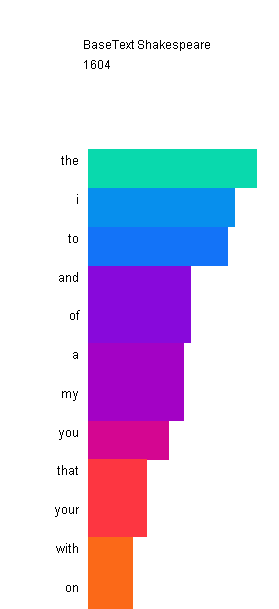
\includegraphics[width=9cm, height=15cm]{Figs/condordanceVis}\\[1ex]
	\caption{The Screen shot of one concordance in the visualisation}
	\label{fig:condorVis}
\end{figure} 

\begin{itemize}
	\item \textbf{String} is drawn to display the term, frequency, version author, publication year; 
	\item \textbf{Rectangle} is used to present the frequency. As the values are sorted in data processing phase, the width of rectangles are set according to these sorted values.
	\item \textbf{Colour} is used to present differences on frequency. Each colour represents a number of frequency, so there will be same colours in different terms.
\end{itemize}

The process in generating the concordance visualization goes through the following steps:
\begin{itemize}
	\item \textbf{} Obtain the string of each term from text source. This step is done in the DataReader class. Detailed illustration seeing Data Reading implementation section.
	\item \textbf{} Calculate the number of times, namely term frequency, of each term occurred in the text (See Data Reading implementation section).  	
	\item \textbf{} Calculate the rectangle width for each term using the frequency of term. The equation of the rectangle width calculating is show in Equation \eqref{rectWidth}:
	
	\begin{multline}\label{rectWidth}
	rectWidth=wordFrequency*unit*scaleValue
	\end{multline}
	
	Where unit is the width of each segment since the rectangle is composed of a number of segments. WordFrequency is the value deciding how many segments compose the rectangle, while scaleValue is the percentage value used to scale the rectangle, range from 10\% to 200\%.
	
	\item \textbf{}Calculate the location of the string and rectangle.The location, or point, is the start drawing point for the string and rectangle. It combined with two point value: point.X, and point.Y. The Equation \eqref{PointX}, \eqref{PointY} illustrate how we calculate these points in the software:
	
	\begin{multline}\label{PointX}
	point.x=versionNumber*versionDistance*scaleValue
	\end{multline}
	
	\begin{multline}\label{PointY}
	point.y= lineNumber*lineDistance*scaleValue
	\end{multline}
	
	Where versionNumber represents order number of the version. versionDistance performs the  distance between two neighbour versions. In addition, a scale value need to be multiplied so that the location of string and rectangle changes according to user preference.
	Similarly, the lineNumber is order number of the term while lineDistance represents the distance between two terms. 
	
	\item \textbf{}Calculate the value of colour. According to \cite{Jbum}, we use the equation as shown in Equation \eqref{Red}: 	
	\begin{multline}\label{Red}
	color = Math.sin(colorFrequency*wordFrequency + phase) * amplitude + center
	\end{multline}
	Where colorFrequency is a constant that controls how fast the wave oscillates. The wordFrequency is  variable used to display different colour according to word frequency. The phase is applied to change the alignment of the green or blue sine waves. The amplitude controls how high (or low) the wave goes. The center controls the center position of the wave.
	
	\item \textbf{}Paint the strings, blocks, and colours by invoking drawing methods in Graphic class. 
	
\end{itemize}

\subsection{Parallel View of Concordances}

Following the generation of concordance visualization, a parallel view of all concordances is created. As shown in Figure \ref{fig:parallelConcor}, all versions of concordances are represented on the panel. During this stage, lines will be drawn to connect same terms. The comparison stage is done in concordancePanel class. 

\begin{figure}[h]
	\centering	
	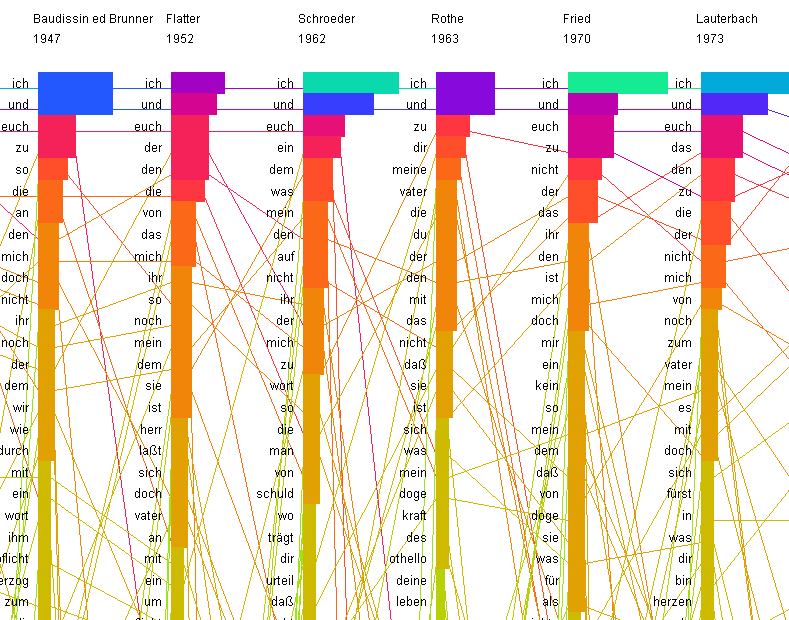
\includegraphics[width=13cm, height=8cm]{Figs/Parallel-Vis}\\[1ex]
	\caption{Parallel view of concordances}
	\label{fig:parallelConcor}
\end{figure} 


However, after this parallel visualization is being generated, an obvious problem appears: there is not enough space for all 16 concordances. So the solution is either to scale the panel, or to select several versions showing one time. We have done both, which are introduced in the following section. 

\subsection{Zooming}

Zooming in and out is a basic feature in the software which designed to provide two zooming options: one is for scaling the content of the visualisation, the other is for scaling the frame. In addition to these two scaling options, there are also scroll bars used to scroll the visualisation panel.

To implement these features, several steps as followed are gone through:
\begin{itemize}
	\item \textbf{} Generate the JSlider objects. This is carried out in the TranslationVisualization class. Figure \ref{fig:jSliders} displays the JSlider applied in the software.
	\begin{figure}[h]
		\centering	
		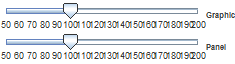
\includegraphics[width=9cm, height=3cm]{Figs/JSliders}\\[1ex]
		\caption{ Sliders applied to zoom in and out the graphic and panel}
		\label{fig:jSliders}
	\end{figure} 	
	\item \textbf{} Obtain scale values from JSlider object and pass them to DataReader class.
	\item \textbf{} Recalculated the data by invoking the calculating methods such as calculatePoint() and setRectWidth().
	\item \textbf{} Update the List<Version> object.
	\item \textbf{} Repaint graphics.
\end{itemize} 
 
During this process, the most difficult part is to recalculate all values of graphics: points, widths and heights for rectangles, and the distances between versions. To overcome this dilemma, two solutions are attempted:
At the first phase, scale() method in Graphics2D class is invoked. By applying this method, computer will calculate and repaint all the graphics using scale parameters passed in. However, when the project prompting to the Term Selecting phase (See Interactive Selection of Terms section below), a problem of obtaining mouse clicking location appears. Hence, the second phase of scaling visualisation comes out.  

At the second phase, scale values attained from JSlider objects are passed to DataReader class and applied in relevant formulas to calculate variables such as points, widths and heights of rectangles. See Equation \eqref{rectWidth}, \eqref{PointX}, and \eqref{PointY}. As shown in \ref{fig:jSliders}, 100 is set as the initial value for the slider, so that the visualisation shown when the visualisation generated at the first time is scaled as 100\%. Figure \ref{fig:zoomIn} and Figure \ref{fig:zoomOut} show the zooming results for the visualisation.

	\begin{figure}[h]
	\centering	
	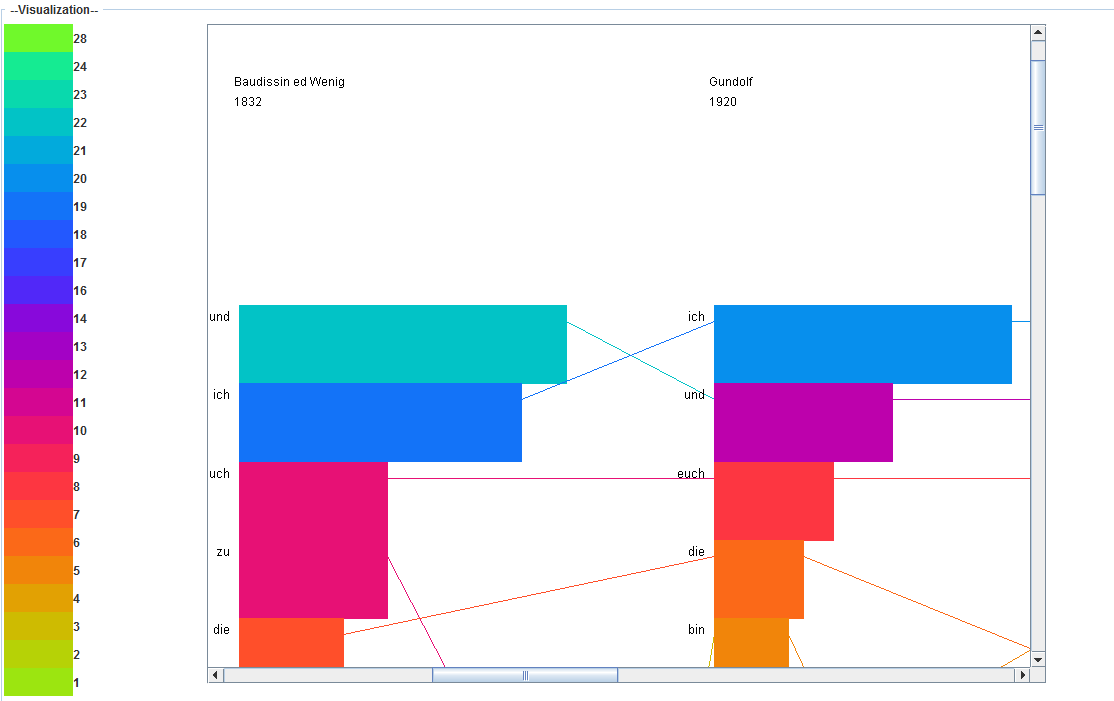
\includegraphics[width=9cm, height=3cm]{Figs/Zoom-In}\\[1ex]
	\caption{}
	\label{fig:zoomIn}
	\end{figure}

	\begin{figure}[h]
	\centering	
	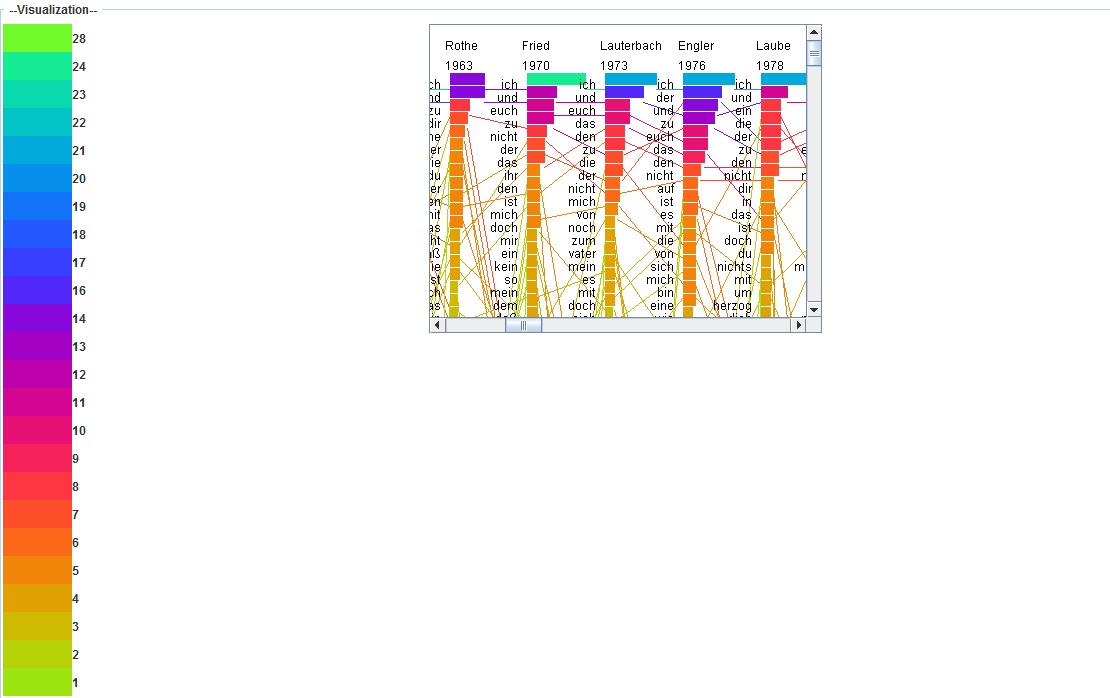
\includegraphics[width=9cm, height=3cm]{Figs/Zoom-Out}\\[1ex]
	\caption{}
	\label{fig:zoomOut}
	\end{figure}

\subsection{Text Labels On and Off}

When the scale values becoming smaller, the strings overlap. Hence a new desire appearing: hide strings on the visualisation. So that users can focus on the rectangles and colours only. 

To implement this feature, a JButton is generated on the panel firstly. Also, "Text On" is set as default label displayed on the button. Secondly, event listener is added to the button. When button is clicked, the label "Text On" on the button will be switched to "Text Off" label. In the meantime, a boolean value which set "true" as default will change to "false", then being given to ConcordancePanel class. In the third step, a boolean value preset when drawing strings of terms will be switched equals to the boolean value passed in. if it is "true", then draw the strings, if it is "false" then not invoke the drawString() method. At last, repaint the graphic. Figure \ref{fig:textOnOff} is a screen shot when we turn off the text.

\begin{figure}[h]
	\centering	
	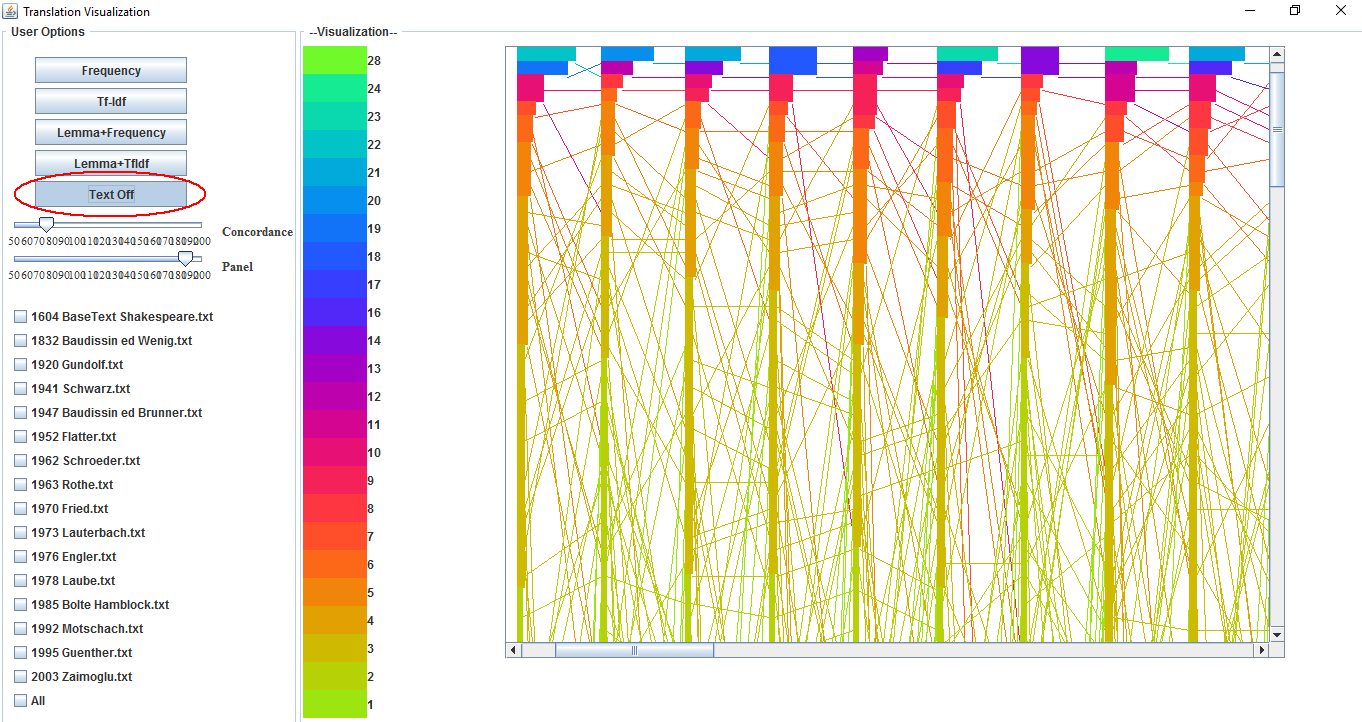
\includegraphics[width=18cm, height=12cm]{Figs/Text-On-Off}\\[1ex]
	\caption{}
	\label{fig:textOnOff}
\end{figure} 

\subsection{Adding, Subtracting, Selecting Items}

To render an user option feature for selecting several concordances displaying on the panel, a new class called VersionChoosenPanel is created. By interacting with this feature, not only can the user select which concordance to display in the visualization, but also the order of concordance displayed can be arranged. Figure
\ref{fig:versionChoosPanel} reveals the menu of version list can be selected. 
\begin{figure}[h]
	\centering	
	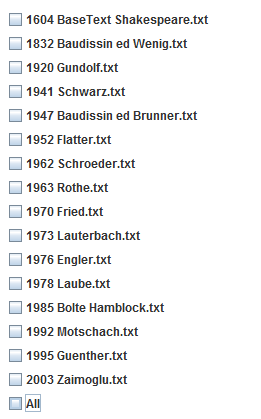
\includegraphics[width=6cm, height=10cm]{Figs/VersionChoosePanel}\\[1ex]
	\caption{The index of version selection}
	\label{fig:versionChoosPanel}
\end{figure} 

The generation of version selection feature goes through the following steps:
\begin{itemize}
	\item \textbf{} Generate a list of JCheckBox class to display the author name as the index. 
	\item \textbf{} Add event listener for each JCheckBox object. So that the action of selection can be generated as an Object class.
	\item \textbf{} Change the selecting status of the index. 
	\item \textbf{} Generate new list of Version objects according to the events passed from JCheckBox ActionListener. Every time the user select a name in the index, a new list of Version objects will be generated and passed to ConcordancePanel class. 
	\item \textbf{} Repaint the concordance visualisation. The ConcordancePanel will be repainted by invoking repaint() method.
	\item \textbf{} Add an option of "All" selection, which is responsible to display or hide all concordances as the original order.
\end{itemize}

Figure \ref{fig:versionChoosDemo}is a screen shot of selecting several versions of concordances to show on the visualisation. Further more, concordances are reordered on the visualisation, where the base text which supposed to be shown as the first version on the left, now being moved to the last one.

\begin{figure}[h]
	\centering	
	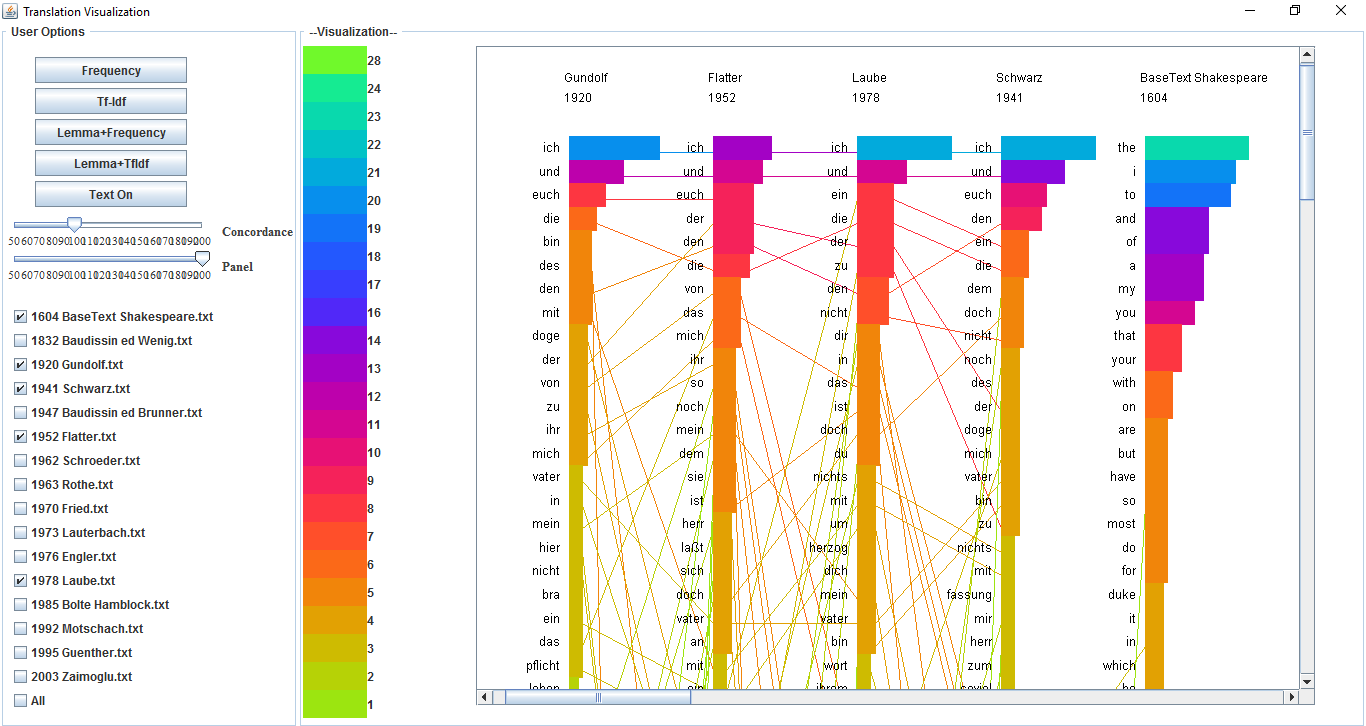
\includegraphics[width=18cm, height=10cm]{Figs/Version-Selecting-Demo}\\[1ex]
	\caption{The screen shot of version selecting feature}
	\label{fig:versionChoosDemo}
\end{figure} 

\subsection{Interaction Selection of Terms}

As each concordance contains a large number of terms, highlight the term following users' options is desired. In order to provide an interactive features for terms, new feature are enable in the visualisation. By achieving these functions, a clear view of term comes out. 

This features are achieved by implementing following phases:
\begin{itemize}
	\item \textbf{}
	\item \textbf{}
	\item \textbf{}
	\item \textbf{}
\end{itemize}

As a result, by clicking one single rectangle in the panel, the rectangle is highlighted and rounded by line while the colour of other rectangles become transparent. In the mean time, lines connecting same terms become highlighted by setting other lines transparent. See Figure \ref{fig:highlightView}

\begin{figure}[h]
	\centering	
	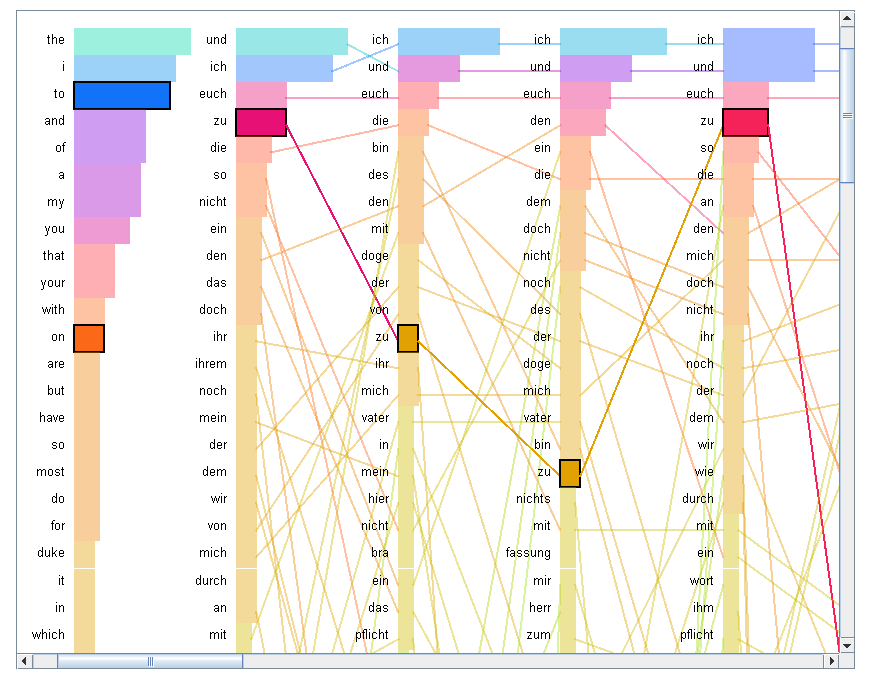
\includegraphics[width=16cm, height=9cm]{Figs/Highlight-Terms}\\[1ex]
	\caption{}
	\label{fig:highlightView}
\end{figure} 

\subsection{Color Mapping}



\subsection{Interactive Color Legend}

\subsection{Lemmatization}
=
\subsection{Tf-Idf}

\subsection{}



